\nsecbegin{Ziel des Sprints}
Ziel des Sprints ist, einen möglichst funktionalen Zwischenstand zu erreichen, der die Spezifikation erfüllt. Insbesondere Unit-Tests für die einzelnen Teile sowie die Weiterentwicklung der Sequenzdiagramm-Generierung sollen implementiert und die Umstrukturierung zu XML  abgeschlossen werden.
Ebenso soll die neue Rahmenstruktur umgesetzt werden.

% HIER NEUES KLASSENDIAGRAMM HINZUFUEGEN
%\begin{figure}[hbtp]
%\centering
%\includegraphics[scale=0.5]{}
%\caption{Klassendiagramm des Sprints}
%\end{figure}
\nsecend

\nsecbegin{User-Stories des Sprint-Backlogs}
\nsecbegin{Klassen- und  Sequenzdiagramme}
\nsecbegin{Auswahl des zu erstellenden Diagramms}
Als Benutzer wünsche ich mir, dass eine Auswahl zwischen Klassen- und Sequenzdiagrammen möglich ist, damit ich diese je nach meinen Bedürfnissen generieren kann.
\nsecend
\nsecbegin{Erstellung von Klassendiagrammen}
Als Benutzer wünsche ich mir, Klassendiagramme aus meinem bestehenden Quellcode erstellen zu können, damit ich einen Überblick über die Klassen meines Programms und deren Beziehungen bekomme.
\nsecend
\nsecbegin{Generierung von Sequenzdiagrammen}
Als Benutzer wünsche ich mir, Sequenzdiagramme erstellen zu können, um einen Überblick über die Abläufe meines Programms zu erhalten.
\nsecend
\nsecend%Klassen- und Sequenzdiagramme
\nsecend % {User-Stories des Sprint-Backlogs}

\nsecbegin{Zeitliche Planung}
\begin{figure}[hbtp]
\centering
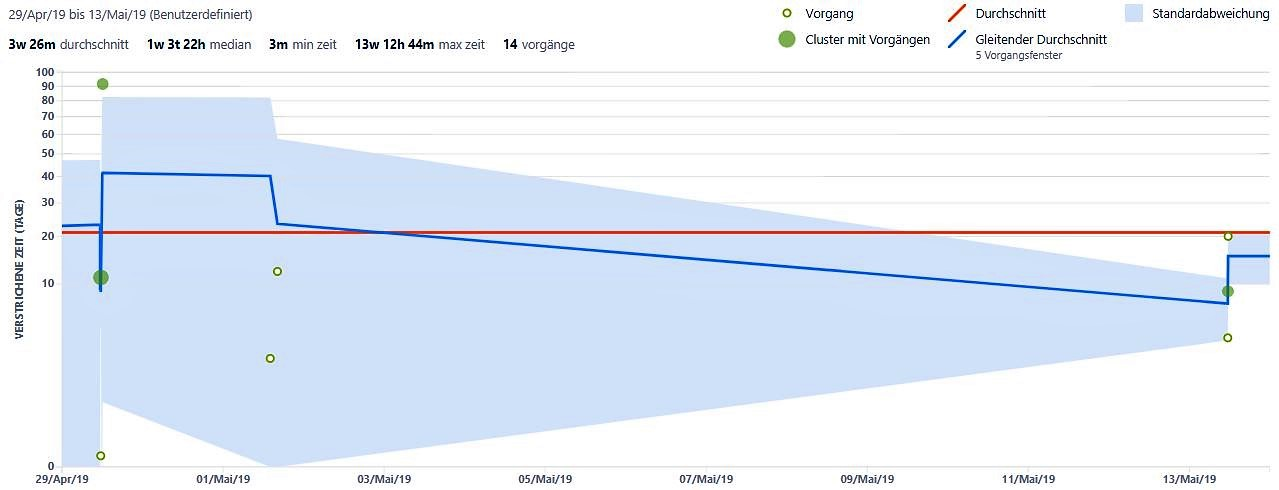
\includegraphics[width=\textwidth]{Bilder/ZeitSprint4}
\caption{Zeit-Diagramm für Sprint 4}
\end{figure}
\nsecend%Zeitliche Planung

\nsecbegin{Liste der durchgeführten Meetings}
\begin{itemize}
\item Planning-Meeting (29.04.2019)
\item Zwischenstandspräsentation (06.05.2019)
\item Zwischen-Meeting (10.05.2019)
\item Review-Meeting (13.05.2019)
\end{itemize}
\nsecend%Liste der durchgeführten Meetings

\nsecbegin{Ergebnisse des Planning-Meetings}
Die XML- und Textspezifikationen sowie deren Transformationen sind allen Teams bekannt. Die Grundlage für die Weiterentwicklung der Sequenzdiagramm-Generierung ist damit gelegt.
\nsecend

\nsecbegin{Aufgewendete Arbeitszeit pro Person$+$Arbeitspaket}
\begin{longtable}{|p{4cm}|l|l|l|l|l|}
        \hline
        Unit-Tests für den Gesamtaufruf & Johann Gerhardt & 01.05.19 & 13.05.19 & 8 & MainTest.java\\
        \hline
        Neue Rahmenstruktur erstellen & Marian Geißler & 29.04.19 & 01.05.19 & 5.5 & Anpassungen an mehreren Klassen\\ 
        \hline
        GUI zu AWT/SWING umbauen & Julian Uebe & 29.04.19 & 13.05.19 & 8 & GUI\_Swing.java\\
		\hline
        Generator für Sequenzdiagramme & Elisabeth Schuster & 29.04.19 & 01.05.19 & 8.5 & SequenzDiagramGenerator.java\\
        \hline
        Generator für Sequenzdiagramme & Leo Rauschke & 29.04.19 & 01.05.19 & 13 & SequenzDiagramGenerator.java\\
        \hline
        & & & & & SequenceDiagramGeneratorTest.java\\
        \hline
        Ausgabe für Sequenz- und Klassendiagramme & Tore Arndt & 07.05.19 & 13.05.19 & 20 & OutputPUML.java\\
        \hline
    	Ausgabe für Sequenz- und Klassendiagramme & Patrick Otte & 29.04.19 & 13.05.19 & 15 & OutputPUML.java\\
    	\hline
    	& & & & & OutputPUMLTest\_classdia.java\\
        \hline
        Generator für Klassendiagramme & Marian Geißler & 29.04.19 & 13.05.19 & 3.5 & ClassDiagramGenerator.java\\
        \hline
        & & & & & XmlHelperMethods.java\\
        \hline
        Generator für Klassendiagramme & Johann Gerhardt & 01.05.19 & 13.05.19 & 16 & ClassDiagramGenerator.java\\
        \hline
        Parser umbauen & Michael Lux & 08.05.19 & 13.05.19 & 14 & ParserJava.java\\
        \hline
        Parser umbauen & Jona Meyer & 08.05.19 & 13.05.19 & 10 & ParserJava.java\\
\hline
\end{longtable}     
\nsecend

\nsecbegin{Konkrete Code-Qualität im Sprint}
Aufgrund der Umstrukturierung sind einige Funktionalitäten noch nicht gegeben. Das Durchlaufen der XML-Bäume sollte teilweise noch angepasst werden. Hierfür bietet sich die Verwendung von XPath-Ausdrücken an.
\nsecend%Konkrete Code-Qualität im Sprint

\nsecbegin{Konkrete Test-Überdeckung im Sprint}
Es fehlen noch viele Unit-Tests und die vorhandenen sollten ausführlicher gestaltet werden.
Ein Gesamttest für das Programm wurde geschrieben.
Die Testüberdeckung ist mit 41,5\% leicht gestiegen.
\nsecend%Konkrete Test-Überdeckung im Sprint

\nsecbegin{Ergebnisse des Reviews}
\begin{table}[H]

\begin{tabularx}{\textwidth}{ |l|l|X| }
\hline
\textbf{Klasse} & \textbf{Methode} & \textbf{Anmerkungen}\\
 \hline
 GUI\_Swing.java & allgemein & Anpassungen\\
 \hline
 SequenzDiagramGenerator.java & Instanzen & Vervollständigung bzgl. Spezifikation + Bugfixing\\
 \hline
 ClassDiagramGenerator.java & createDiagram & Vervollständigung bzgl. Spezifikation + Bugfixing\\
 \hline
 OutputPUML.java & getPUML & Output für Sequenzdiagramme anpassen\\
 \hline
 XmlHelperMethods.java & allgemein & weitere nützliche Methoden in die Klasse überführen\\
 \hline
 ParseJava.java & allgemein & Vervollständigung bzgl. Spezifikation + Bugfixing\\
%Console & showConsole & Pfad anpassen \\
\hline
\end{tabularx}
\end{table}

Sonstiges:
\begin{itemize}
\item XPath nutzen
\item Rekursive Implementierung beim Abarbeiten von verschachtelten Elementen
\item Fehlende Unit-Tests nachholen
\item Evtl. in späterem Sprint: Handling von Methoden in Bedingungen
\end{itemize}
\nsecend%Ergebnisse des Reviews

\nsecbegin{Abschließende Einschätzung des Product-Owners}
Die Funktionalität nach diesem Sprint lässt noch zu wünschen übrig, es bestehen viele Teile der Spezifikation, die noch nicht erfüllt sind.
\nsecend%Abschließende Einschätzung des Product-Owners

\nsecbegin{Abschließende Einschätzung des Software-Architekten}
Das Projekt befindet sich immer noch im Umbau. Einzelne Module sind bereits lauffähig.
\nsecend%Abschließende Einschätzung des Software-Architekten